\documentclass[11pt,a4paper]{article}
\usepackage[T1]{fontenc}
\usepackage[utf8]{inputenc}
\usepackage[english]{babel}
\usepackage[margin=27mm,headheight=15pt]{geometry}
\usepackage{amsmath}
\usepackage{newtxtext,newtxmath}
\usepackage{microtype}
\usepackage{graphicx}
\usepackage{xcolor}
\usepackage{booktabs,array,tabularx,longtable}
\usepackage{caption,subcaption}
\usepackage{setspace}
\usepackage{enumitem}
\usepackage[section]{placeins}
\usepackage{fancyhdr}
\usepackage{titlesec}
\usepackage[numbers,sort&compress]{natbib}
\usepackage{xurl}
\usepackage{hyperref}

\definecolor{thesisblue}{HTML}{193952}
\definecolor{thesisgray}{HTML}{657381}
\hypersetup{colorlinks=true,linkcolor=thesisblue,citecolor=thesisblue,
  urlcolor=thesisblue,pdftitle={Unsupervised Deep Clustering of Multivariate Particle Trajectories in PIC Simulations}}
\urlstyle{same}
\setstretch{1.12}
\setlength{\parindent}{1.25em}
\setlength{\parskip}{0.3em}
\setlength{\emergencystretch}{2em}
\clubpenalty=10000
\widowpenalty=10000
\displaywidowpenalty=10000
\setlength{\tabcolsep}{5pt}
\renewcommand{\arraystretch}{1.2}
\newcolumntype{Y}{>{\raggedright\arraybackslash}X}
\captionsetup{font=small,labelfont=bf,skip=8pt}
\captionsetup[subfigure]{font=small,justification=centering}
\setlist[itemize]{nosep,topsep=0.4em,leftmargin=1.5em}
\titleformat{\section}{\Large\bfseries\color{thesisblue}}{\thesection}{0.7em}{}
\titleformat{\subsection}{\large\bfseries}{\thesubsection}{0.7em}{}
\titlespacing*{\section}{0pt}{1.2em}{0.8em}
\titlespacing*{\subsection}{0pt}{1em}{0.4em}
\numberwithin{equation}{section}
\setcounter{tocdepth}{2}
\renewcommand{\topfraction}{0.9}
\renewcommand{\bottomfraction}{0.8}
\renewcommand{\textfraction}{0.08}
\renewcommand{\floatpagefraction}{0.65}
\pagestyle{fancy}
\fancyhf{}
\fancyhead[L]{\small\textit{Multivariate PIC Trajectory Clustering}}
\fancyhead[R]{\small Internship report}
\fancyfoot[C]{\thepage}
\renewcommand{\headrulewidth}{0.3pt}
\fancypagestyle{plain}{\fancyhf{}\fancyfoot[C]{\thepage}\renewcommand{\headrulewidth}{0pt}}

\newcommand{\placeholder}[2][38mm]{%
  \begingroup\setlength{\fboxsep}{7pt}%
  \fcolorbox{thesisgray}{white}{%
    \parbox[c][#1][c]{\dimexpr\linewidth-2\fboxsep-2\fboxrule\relax}{%
      \centering\small\color{thesisgray}#2}}%
  \endgroup}
\newcommand{\figureasset}[3][0.95\linewidth]{%
  \IfFileExists{#2}{\includegraphics[width=#1,height=0.7\textheight,keepaspectratio]{#2}}%
    {\placeholder[55mm]{#3\\[0.5em]Image to be supplied}}}

\newcommand{\thesistitle}{Unsupervised Deep Clustering of\\Multivariate Particle Trajectories\\in PIC Simulations}
\newcommand{\studentname}{Linshuo CHEN}
\newcommand{\universityname}{Sorbonne Universit\'e}
\newcommand{\masterprogram}{M2 -- Parcours Statistique, apprentissage et algorithmes}
\newcommand{\internshipsupervisor}{Andrea CIARDI}
\hypersetup{pdfauthor={\studentname},pdfsubject={M2 Internship report}}

\begin{document}
\hypersetup{pageanchor=false}
\begin{titlepage}
\thispagestyle{empty}
\centering
\vspace*{0.4cm}

\includegraphics[width=0.43\textwidth]{figures/sorbonne-universite.png}\par
\vspace{2.1cm}
{\fontsize{17}{23}\selectfont\masterprogram\par}
\vspace{0.9cm}
{\Large\scshape Internship report\par}
\vspace{1.2cm}
\rule{\linewidth}{0.4pt}\par
\vspace{0.6cm}
{\fontsize{25}{32}\selectfont\mdseries\thesistitle\par}
\vspace{0.6cm}
\rule{\linewidth}{0.4pt}\par
\vspace{2.0cm}
\begin{minipage}[t]{0.34\textwidth}
\raggedright\Large
\textbf{\textit{Author:}}\par
\vspace{0.3em}
\studentname
\end{minipage}\hspace{0.08\textwidth}%
\begin{minipage}[t]{0.34\textwidth}
\raggedleft\Large
\textbf{\textit{Supervisor:}}\par
\vspace{0.3em}
\internshipsupervisor
\end{minipage}\par
\vfill
\end{titlepage}
\hypersetup{pageanchor=true}
\pagenumbering{roman}
\section*{Abstract}
\addcontentsline{toc}{section}{Abstract}

Particle-in-cell (PIC) simulations produce large datasets of particle trajectories that require automated methods for grouping and analysis. This internship adapts a previous spectrogram-based deep clustering workflow to six-channel records comprising particle position, momentum components, and local electromagnetic fields. The study uses 12,800 particles. After temporal subsampling and channel-wise standardization, the time series are converted into log-magnitude spectrograms. A convolutional autoencoder learns 32-dimensional representations, which are used for K-means initialization and deep clustering refinement with a reconstruction constraint. An elbow criterion selects five clusters from a candidate range of two to twelve. The method is compared with PCA followed by K-means on the same spectrogram inputs and a one-dimensional convolutional autoencoder with clustering refinement operating on standardized time series. On a common sample of 10,000 particles, the silhouette scores are 0.29957 for PCA + K-means, 0.79637 for the time-series method, and 0.87985 for the spectrogram method.  
\clearpage
\begingroup
\small\setstretch{1.0}
\setlength{\parskip}{0pt}
\tableofcontents
\endgroup
\clearpage
\phantomsection
\addcontentsline{toc}{section}{List of Figures}
\listoffigures
\bigskip
\phantomsection
\addcontentsline{toc}{section}{List of Tables}
\listoftables
\clearpage
\pagenumbering{arabic}

\section{Introduction}\label{sec:introduction}

Particle-in-cell (PIC) simulations are a useful numerical method for the study of plasma dynamics since they can record particle positions, momenta, and electromagnetic fields, which are sampled along particle trajectories, thus generating large sets of multivariate time series. As the number of tracked particles, recorded time steps, and available variables increases, it becomes insufficient to examine individual trajectories or to compare a small number of two-dimensional projections for systematic analysis. For this reason, automated feature extraction and the grouping of particles with similar trajectory characteristics constitute an important aspect of PIC data analysis.

Unsupervised learning allows this task to be carried out without the need for previously defined particle labels. By constructing suitable data representations and grouping samples by similarity, large trajectory datasets can be organized into more manageable subsets. Markidis et al. introduced an automated workflow for classifying particle trajectories from plasma simulations by combining the fast Fourier transform, principal component analysis, K-means clustering, and silhouette analysis. This method was applied to electron trajectories in a magnetic reconnection simulation, which laid the foundation for the investigation of particle trajectory datasets using dimensionality reduction and clustering~\cite{markidis2020}.

Deep representation learning offers another approach to processing complex trajectory data. Autoencoders learn low-dimensional features through an input reconstruction task, so that high-dimensional samples can be represented in a compact space. Deep Embedded Clustering (DEC) combines representation learning with cluster assignment, iteratively modifying both the feature representation and the positions of the cluster centers in order to achieve the clustering aim. This method provides a framework in which the representation used to group samples is learned from the data~\cite{xie2016}.

The present study is based on the internship report \textit{Exploring Particle In Cell Simulation Data Using Artificial Intelligence} by Medina Moreira. That work looked into unsupervised particle trajectory analysis using position and kinetic energy time series, spectrogram representations, convolutional autoencoders, and deep clustering. It also pointed out that there was a lack of information regarding momentum and the electromagnetic fields in the dataset and proposed that the workflow be extended by including further variables as input channels. This suggestion from the report serves as the foundation for the present study, which applies the existing framework to more comprehensive descriptions of particle trajectories and investigates the related data processing and clustering performance~\cite{moreiraReport}.

Extending the input to additional variables leads to further data-processing challenges. Since position, momentum, and electromagnetic fields have different numerical scales and temporal characteristics, their relative contributions are sensitive to preprocessing. The inclusion of more variables also raises the dimensionality of each sample and may result in correlated or redundant information. Therefore, channel normalization, feature extraction, and clustering evaluation must be considered together when constructing a multivariate trajectory representation. Following the previous workflow, this study uses spectrograms to represent the evolution of local frequency content within each time series. The spectrograms of different variables are combined into a multichannel input for feature learning with a convolutional autoencoder.

The input variables considered here comprise particle position \(x\), momentum components \(p_x\) and \(p_y\), electric field components \(E_x\) and \(E_y\), and the magnetic field component \(B_z\), with the fields recorded along particle trajectories. The workflow begins by normalizing the variables and then transforms the time-series data into spectrograms. A convolutional autoencoder is then used to learn low-dimensional representations, which are used to initialize cluster centers through K-means. Subsequent deep clustering refinement retains a reconstruction constraint while updating both the representation and cluster assignments. The spectrogram-based workflow determines the number of clusters using an elbow criterion. This selected value is then applied to the reference methods so that the number of clusters remains consistent across the comparisons.

\begin{figure}[htbp]
\centering
\figureasset[\linewidth]{figures/workflow-no-trajectories.png}{Overview of the multivariate PIC deep clustering workflow}
\caption[Overview of the multivariate PIC deep clustering workflow]{Overview of the spectrogram-based deep clustering workflow for multivariate PIC particle trajectories. Time series of particle position, momentum components, and local electromagnetic fields are normalized and transformed into multichannel log-spectrograms. A convolutional autoencoder learns latent representations, from which the number of clusters is selected using an elbow criterion. K-means initialization is followed by deep clustering refinement with a reconstruction constraint to obtain the final cluster assignments. Clustering quality is evaluated primarily using the silhouette score, with reconstruction errors, visualizations, and cluster statistics providing supplementary diagnostics. All plots are schematic.}\label{fig:workflow}
\end{figure}

Because predefined particle labels are unavailable, clustering quality is mainly assessed through internal validation. The silhouette score is used as the main evaluation metric. This score measures both cohesion within clusters and separation between clusters by comparing, for each sample, its distances to samples in its own cluster and to those in its nearest neighboring cluster~\cite{rousseeuw1987}. Its interpretation depends on the feature space and distance metric used for evaluation. Supplementary diagnostic information is obtained from reconstruction errors, cluster-size distributions, and dimensionality-reduction visualizations. As a reference approach to help assess the effect of the spectrogram representation, a one-dimensional convolutional autoencoder that operates directly on the original time series is included. A further linear baseline is provided by PCA followed by K-means using the same spectrogram inputs as the main method.

This study aims to apply the earlier spectrogram-based deep clustering procedure to multivariate particle data and to evaluate its capabilities in terms of feature extraction and clustering. The rest of the report is structured as follows. Section~\ref{sec:data} deals with the dataset, input variables, and preprocessing methods. Section~\ref{sec:methodology} presents the construction of multichannel spectrograms, the convolutional autoencoder, the deep clustering procedure, and the strategy for selecting the number of clusters. Section~\ref{sec:experiments} sets out the experimental design and evaluation method. Section~\ref{sec:results} presents the clustering results together with additional diagnostic information. Section~\ref{sec:conclusions} contains the conclusions, limitations, and implications. Section~\ref{sec:ai-assistance} provides the declaration of AI assistance. Further details regarding the architecture and training settings are given in Appendix~\ref{app:implementation}, and the final cluster statistics are listed in Appendix~\ref{app:clusters}.

\clearpage
\section{Data and Problem Definition}\label{sec:data}

\subsection{Data Source and Organization}

This study uses the research project's PIC particle-tracking data to examine unsupervised clustering of multivariate particle trajectories. The dataset is stored in HDF5 format and includes records of particle position, momentum components, and electromagnetic field components for 12,800 particles across 6,010 recorded time points.

The variables are arranged as two-dimensional arrays of size \(6010 \times 12800\), with the first dimension corresponding to time and the second to particles. A shared time array specifies the recording times, while particle identifiers associate the variables and clustering results with individual particles. Variable names, coordinate components, and numerical conventions follow those of the provided dataset.

Each analysis sample consists of the multivariate time series for one particle over the entire recording interval. The same time indices are applied to all variables to ensure correspondence between the different channels. Particle identifiers are retained to track samples and link the outputs with the original records; they are not employed as input features or as predefined class labels.

\subsection{Input Variables and Multichannel Representation}

The previous study based its clustering inputs mainly on particle position and kinetic energy time series and suggested extending the workflow to include momentum and electromagnetic field information. The current study follows this approach by modifying the input representation to incorporate these additional particle data types~\cite{moreiraReport}.

The main configuration uses six input channels: \(x\), \(p_x\), \(p_y\), \(E_x\), \(E_y\), and \(B_z\), as summarized in Table~\ref{tab:channels}. The available \(p_z\) component is not included in this configuration.

\begin{table}[htbp]
\centering\small
\caption{Input channels used for multivariate particle trajectory clustering.}\label{tab:channels}
\begin{tabularx}{\linewidth}{@{}p{0.18\linewidth}p{0.1\linewidth}Y@{}}
\toprule
\textbf{Category} & \textbf{Variable} & \textbf{Description} \\
\midrule
Position & \(x\) & Particle position along the \(x\)-axis \\
Momentum & \(p_x\) & \(x\)-component of particle momentum \\
Momentum & \(p_y\) & \(y\)-component of particle momentum \\
Electric field & \(E_x\) & Electric field component along \(x\), recorded along the particle trajectory \\
Electric field & \(E_y\) & Electric field component along \(y\), recorded along the particle trajectory \\
Magnetic field & \(B_z\) & Magnetic field component along \(z\), recorded along the particle trajectory \\
\bottomrule
\end{tabularx}
\end{table}

Each channel contains the temporal evolution of a single variable, and together the six channels describe an individual particle during the recording interval. Since the variables differ in numerical scale, fluctuation amplitude, and temporal behavior, a common data-organization procedure and channel-specific standardization are required.

Figure~\ref{fig:time-series} presents the standardized six-channel time series of the first five particles in the dataset. The same color identifies the same particle in every panel. These examples illustrate the input structure and temporal variation across channels; they are not selected as representatives of the resulting clusters.

\begin{figure}[htbp]
\centering
\figureasset[\linewidth]{figures/time-series.png}{Standardized six-channel time series for five particles}
\caption[Standardized six-channel time series for five particles]{Standardized six-channel time series for five example particles. The panels show \(x\), \(p_x\), \(p_y\), \(E_x\), \(E_y\), and \(B_z\) for the first five particles in the dataset. Particle indices 0--4 correspond to identifiers 1--5, and the same color denotes the same particle across all panels. Each channel is standardized using its mean and standard deviation across all particles and selected time points. The horizontal axis gives the sample index after fixed-stride subsampling, yielding 2,004 points separated by 1200 in the dataset's recorded time convention.}\label{fig:time-series}
\end{figure}

\subsection{Uniform Temporal Sampling and Standardization}

The original time array extends from 0 to 2,403,600, with a constant interval of 400 between consecutive records. These values follow the time convention of the supplied dataset. To reduce the computational cost of constructing the spectrograms and training the model, a fixed stride of three is applied when selecting records. This produces 2,004 time points with a uniform interval of 1200, while retaining both the first and last recording times for the current dataset.

The same sampling indices are applied to every particle and channel, ensuring that temporal order and correspondence between variables are maintained. Sampling selects existing recorded values directly, without interpolation. Each particle is therefore represented by a multichannel time-series array of size \(6 \times 2004\).

Before spectrogram construction, each channel is standardized to account for differences in numerical scale. The mean and standard deviation are calculated across all 12,800 particles and all 2,004 selected time points for that channel. Values are then transformed by subtracting the channel mean and dividing by its standard deviation. All particles within a channel share a single pair of standardization parameters, rather than each particle being normalized independently.

This procedure produces dimensionless standardized values while preserving relative amplitude differences between particles within the same channel. The time series in Figure~\ref{fig:time-series} use the same standardization parameters as those used for spectrogram construction. Since these parameters are based on the entire analysis dataset, this preprocessing configuration supports exploratory clustering of the supplied dataset.

\subsection{Spectrogram Representation and Clustering Task}

The standardized time series are converted into log-magnitude spectrograms separately for each channel. After resizing and channel-wise standardization in the spectrogram domain, the resulting arrays form the input to the convolutional autoencoder. Each channel is represented on a \(33 \times 60\) grid, giving an input tensor of size \(6 \times 33 \times 60\) for each particle.

The six channels correspond to the selected variables, while the other two dimensions represent the resized frequency and time axes. Together, these dimensions define the network input grid and do not indicate the actual numbers of independent frequency bins and time windows in the original transform. Spectrogram computation uses a sampling frequency of one, with frequency expressed in cycles per sampled point. Details of the transform parameters and resizing procedure are provided in Section~\ref{sec:methodology}.

The clustering task aims to partition particle trajectories into groups using these multichannel representations when no predefined class labels are available. Treating each individual trajectory as a sample and grouping them through feature extraction and clustering follows the general task formulation used in earlier PIC trajectory classification studies~\cite{markidis2020}.

For the entire analysis interval, each particle is assigned a single final cluster label and does not receive separate labels for individual temporal segments. Cluster indices identify the groups formed and have no predefined class names or ordering. The convolutional autoencoder learns a low-dimensional representation, which is then used for cluster initialization and refinement. In this report, the spectrogram-based approach determines the number of clusters within the candidate range \(K=2,\ldots,12\) using an elbow criterion; the selected value, \(K=5\), is then fixed for both reference methods.

\subsection{Clustering Evaluation}

Because reference class labels are unavailable, clustering is evaluated through internal validation, with the silhouette score serving as the primary metric. For each sample, this score compares the average distance to other samples in its own cluster with the average distance to samples in the nearest neighboring cluster, thereby measuring within-cluster cohesion and between-cluster separation~\cite{rousseeuw1987}.

Silhouette scores are computed using Euclidean distances in the learned latent space, with subsampling used to limit computational cost. Higher silhouette scores indicate more compact and separated groups under the chosen representation and distance metric. Although the score describes clustering structure, it is not interpreted as a measure of classification accuracy relative to ground-truth labels.

Reconstruction errors provide additional information about the model's ability to reproduce its inputs, cluster-size distributions show how particles are allocated among the groups, and PCA and t-SNE visualizations help display the learned feature structure. Detailed evaluation settings and quantitative results are provided in Section~\ref{sec:experiments} and Section~\ref{sec:results}, respectively.

\clearpage
\section{Methodology}\label{sec:methodology}

\subsection{Overview}

This study uses an unsupervised deep clustering procedure that is based on multichannel spectrograms in order to extract features from particle trajectories and to automatically group particles. The workflow includes spectrogram construction, convolutional autoencoder pretraining, cluster-count selection and initialization, and deep clustering refinement with a reconstruction constraint.

This method is based on earlier work that involved the use of spectrograms and convolutional autoencoders for particle time-series analysis and adapts the input to six channels containing position, momentum, and electromagnetic field information~\cite{moreiraReport}. First, the standardized time series described in Section~\ref{sec:data} are converted into multichannel spectrograms. A reconstruction task then learns low-dimensional features, and then the number of clusters and initial cluster centers are determined. Finally, the representation and the assignment of particles are then improved by jointly optimizing the reconstruction and clustering losses.

The overall workflow is shown in Figure~\ref{fig:workflow}.

\subsection{Multichannel Spectrogram Construction}

A spectrogram is computed separately for each of the six standardized time series associated with each particle. The implementation uses the SciPy spectrogram function with a window length of 256 samples and a hop size of 128 samples, corresponding to 50\% overlap between adjacent windows. A Tukey window with a shape parameter of 0.25 is used, and the mean is removed within each window. A one-sided magnitude spectrum is returned. The sampling frequency is set to one, so frequencies are expressed in cycles per sampled point~\cite{scipySpectrogram}.

The magnitude spectrum is transformed according to

\begin{equation} S_{\log}=\log(1+S), \end{equation}

where \(S\) denotes the magnitude spectrum. This transformation compresses its numerical dynamic range before network processing.

For a time series with 2,004 samples, these settings produce 129 frequency bins and 14 time windows. Only complete windows are used, without padding at the end of the sequence; the leftover samples do not constitute an extra frame. Bilinear interpolation subsequently resizes the log-magnitude spectrogram to a fixed \(33\times60\) grid. This resampling process acts on the existing representation and does not add any new independent temporal or spectral information.

The resized spectrograms are standardized separately for each channel by the mean and standard deviation computed across all particles and all spectrogram grid points in that channel. The six channels are then combined into an input tensor of size \(6\times33\times60\) for each particle. Figure~\ref{fig:spectrogram} illustrates the resulting six-channel input for one particle.

\begin{figure}[htbp]
\centering
\figureasset[\linewidth]{figures/input-log-spectrogram-example.png}{Six-channel spectrogram input for an example particle}
\caption[Six-channel spectrogram input for an example particle]{Six-channel spectrogram input for an example particle. The panels correspond to \(x\), \(p_x\), \(p_y\), \(E_x\), \(E_y\), and \(B_z\). Each time series is transformed into a magnitude spectrogram, logarithmically compressed, resized, and standardized channel-wise to form the convolutional autoencoder input. The horizontal and vertical axes indicate the resized time-bin and frequency-bin indices, respectively. Colors represent standardized log-magnitude values, with an independent color scale for each panel.}\label{fig:spectrogram}
\end{figure}

\subsection{Convolutional Autoencoder and Reconstruction Pretraining}

The convolutional autoencoder has an encoder and a decoder. The encoder compresses the multichannel spectrogram into a low-dimensional feature vector, and the decoder reconstructs the input from that vector. The feature representation used for the subsequent clustering is obtained by minimizing the reconstruction error.

For particle \(i\), let \(X_i\) denote its six-channel spectrogram input. With encoder \(f_\theta\) and decoder \(g_\phi\), the latent representation and reconstruction are

\begin{equation} z_i=f_\theta(X_i), \qquad \widehat{X}_i=g_\phi(z_i), \end{equation}

where \(z_i\in\mathbb{R}^{32}\), and \(\theta\) and \(\phi\) are the trainable encoder and decoder parameters, respectively.

The encoder contains four two-dimensional convolutional layers with 8, 16, 32, and 64 output channels. Each layer uses a \(3\times3\) kernel, a stride of two, padding of one, and a ReLU activation. The final convolutional output is flattened and mapped to a 32-dimensional feature vector through a linear fully connected layer.

The decoder first maps the latent vector back to the convolutional feature dimensions through a fully connected layer. Four transposed convolutional layers then reconstruct the multichannel representation. ReLU activations follow the first three transposed convolutional layers, while the final layer has no non-negative activation constraint, and thus is able to reconstruct standardized inputs that include negative values. Bilinear interpolation adjusts the output to the original input dimensions. A summary of the main architecture can be found in Table~\ref{tab:architecture} in Appendix~\ref{app:implementation}.

Pretraining minimizes a channel-weighted mean squared error:

\begin{equation} L_{\mathrm{recon}} = \frac{ \displaystyle \sum_{i\in\mathcal{B}} \sum_{c=1}^{C} w_c \left\|\widehat{X}_{i,c}-X_{i,c}\right\|_F^2 }{ BHW\displaystyle\sum_{c=1}^{C}w_c }, \end{equation}

where \(\mathcal{B}\) denotes the current batch, \(B\) is its number of samples, \(C=6\) is the number of channels, and \(H=33\) and \(W=60\) are the spectrogram grid dimensions. The squared Frobenius norm sums the squared reconstruction errors over all grid points within a channel.

For the channel ordering \(x,p_x,p_y,E_x,E_y,B_z\), the weights are

\begin{equation} \boldsymbol{w}=(1,\;1,\;1,\;0.2,\;0.2,\;1). \end{equation}

This configuration reduces the relative contribution of electric-field reconstruction errors to the training objective while retaining all six channels as inputs.

During pretraining, particles are randomly divided into an 80\% training subset and a 20\% validation subset, which contain 10,240 and 2,560 particles, respectively. Training uses the Adam optimizer with a learning rate of \(10^{-3}\), a batch size of 64, and a maximum of 200 epochs. Pretraining stops when the validation loss has not improved for 15 consecutive epochs. The model with the lowest validation loss is selected for subsequent clustering.

This split is used to monitor reconstruction training. The fact that the standardization parameters are calculated from the whole analysis dataset means that the validation subset is not regarded as an independent generalization test set.

\subsection{Cluster-Count Selection and Initialization}

After pretraining, the encoder extracts 32-dimensional features for all particles. \(K\)-means is then used in this feature space for each possible number of clusters \(K\) ranging from 2 to 12. For each candidate configuration, there are 100 initializations, and each initialization is carried out for a maximum of 1,000 iterations. The solution that has the smallest within-cluster sum of squared distances is kept.

For a candidate cluster count \(K\), the \(K\)-means inertia is

\begin{equation} I(K) = \sum_{i=1}^{N} \left\|z_i-\mu_{a_i}\right\|_2^2, \end{equation}

where \(N\) is the number of particles, \(a_i\) is the \(K\)-means assignment of particle \(i\), and \(\mu_{a_i}\) is the corresponding cluster center.

The elbow criterion, which is based on log inertia, is used to determine the number of clusters. The proposed numbers of clusters and their corresponding log-inertia values are each rescaled independently to the range \([0,1]\). Then the perpendicular distance from each of the resulting points to the line joining the first and last of the candidate points is calculated, and the candidate having the greatest distance is chosen as the elbow.

Silhouettes are also calculated for the candidate configurations as additional information; the maximum of these values is not employed in determining \(K\). After the number of clusters has been chosen, the respective \(K\)-means centers are used to initialize the deep clustering layer.

Figure~\ref{fig:cluster-count-selection} shows the corresponding diagnostics for the pretrained spectrogram representation. The elbow criterion selects \(K=5\), which does not maximize the sampled silhouette score over the candidate range. These silhouette values describe \(K\)-means assignments before DEC refinement and are distinct from the final clustering scores reported in Section~\ref{sec:silhouette-results}.

\begin{figure}[htbp]
\centering
\begin{subfigure}[t]{0.49\linewidth}
\centering
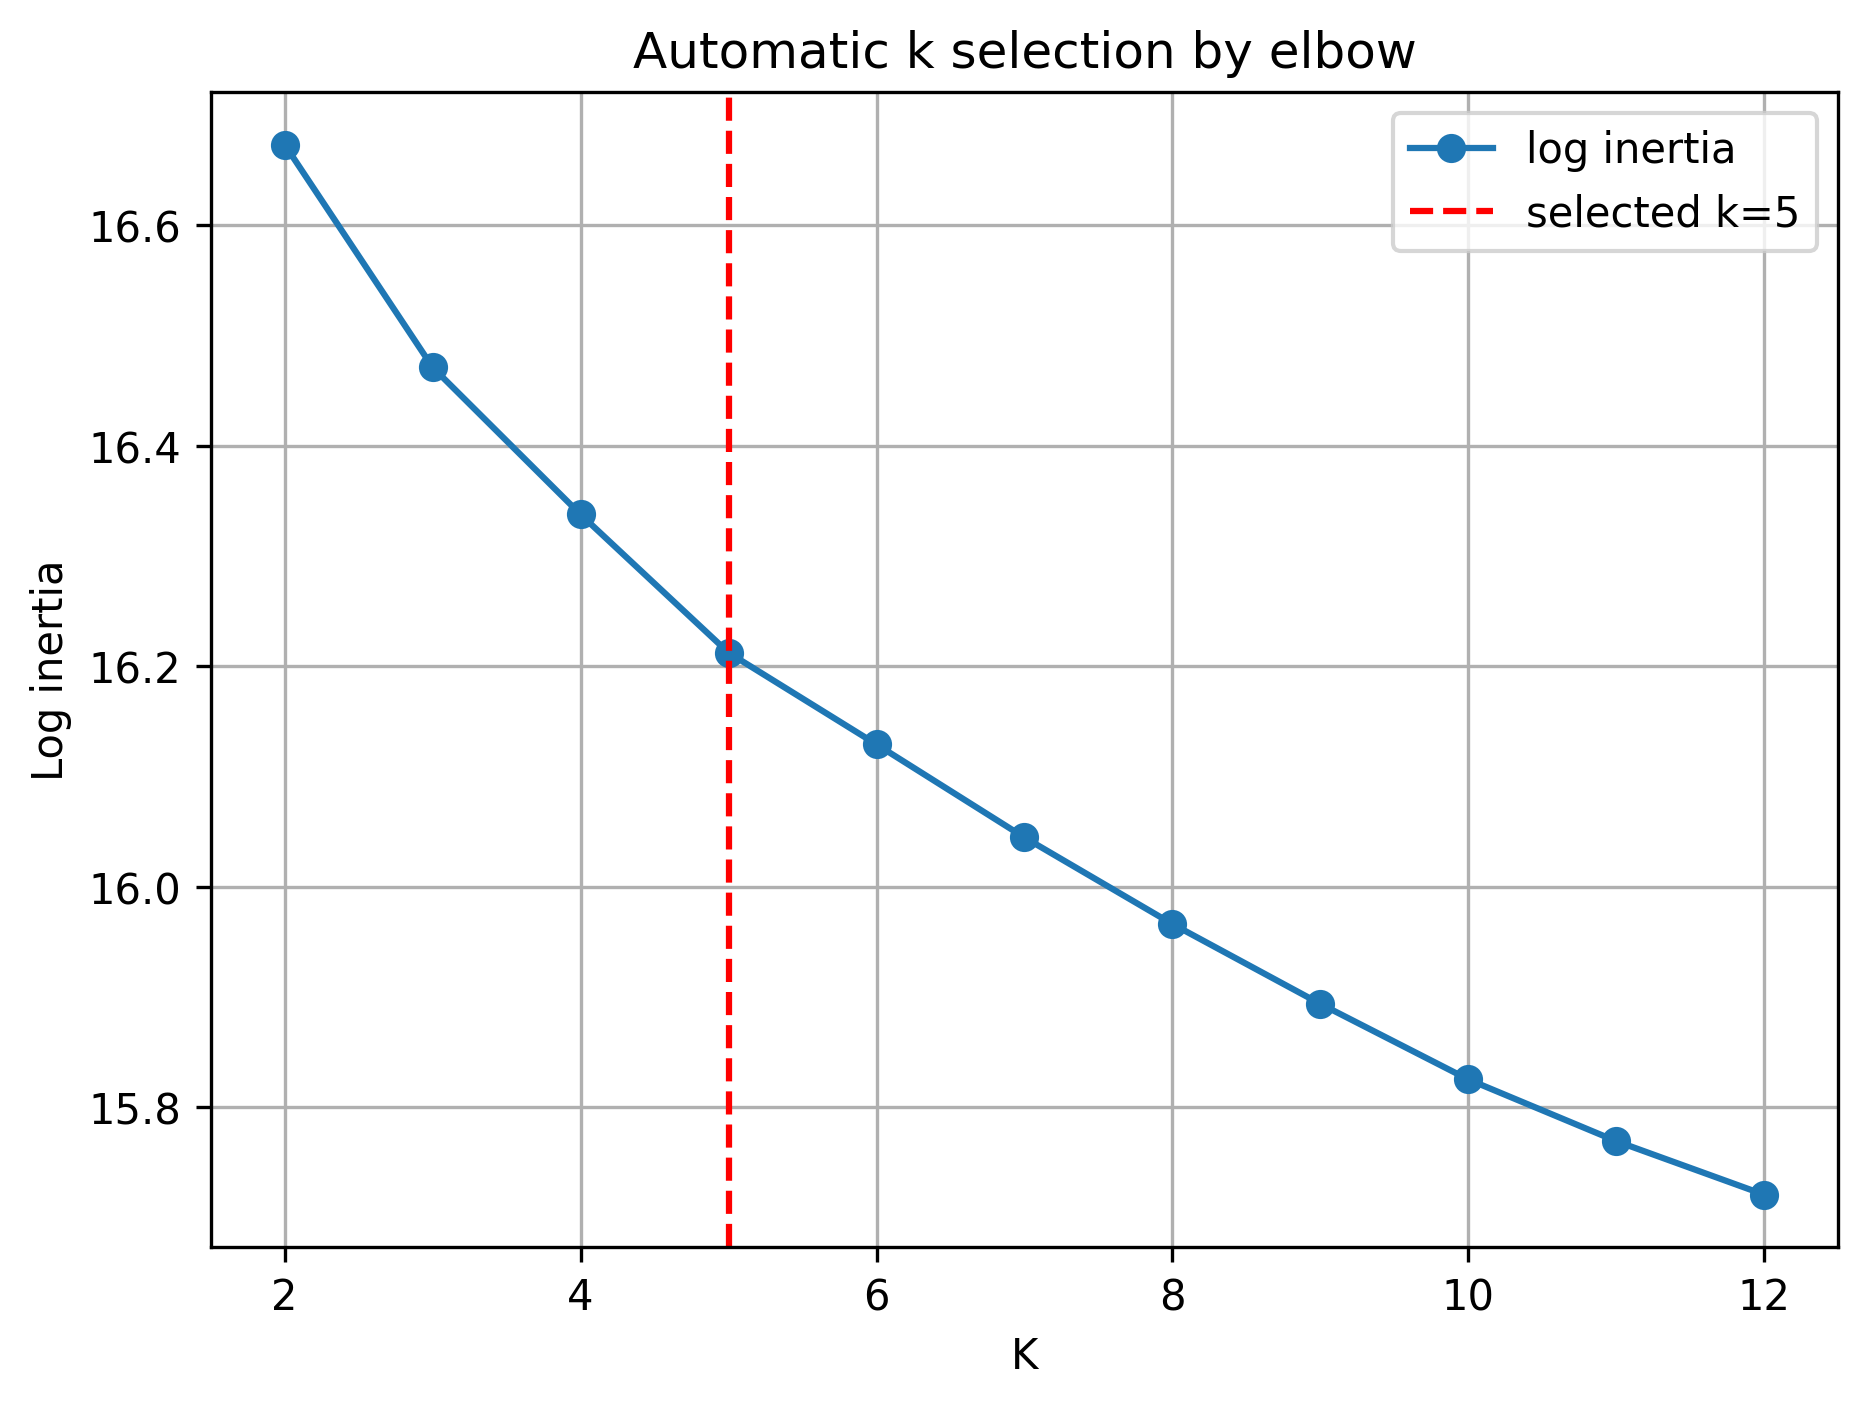
\includegraphics[width=\linewidth]{figures/cluster-count-elbow.png}
\caption{Log inertia and elbow-selected cluster count.}
\end{subfigure}\hfill
\begin{subfigure}[t]{0.49\linewidth}
\centering
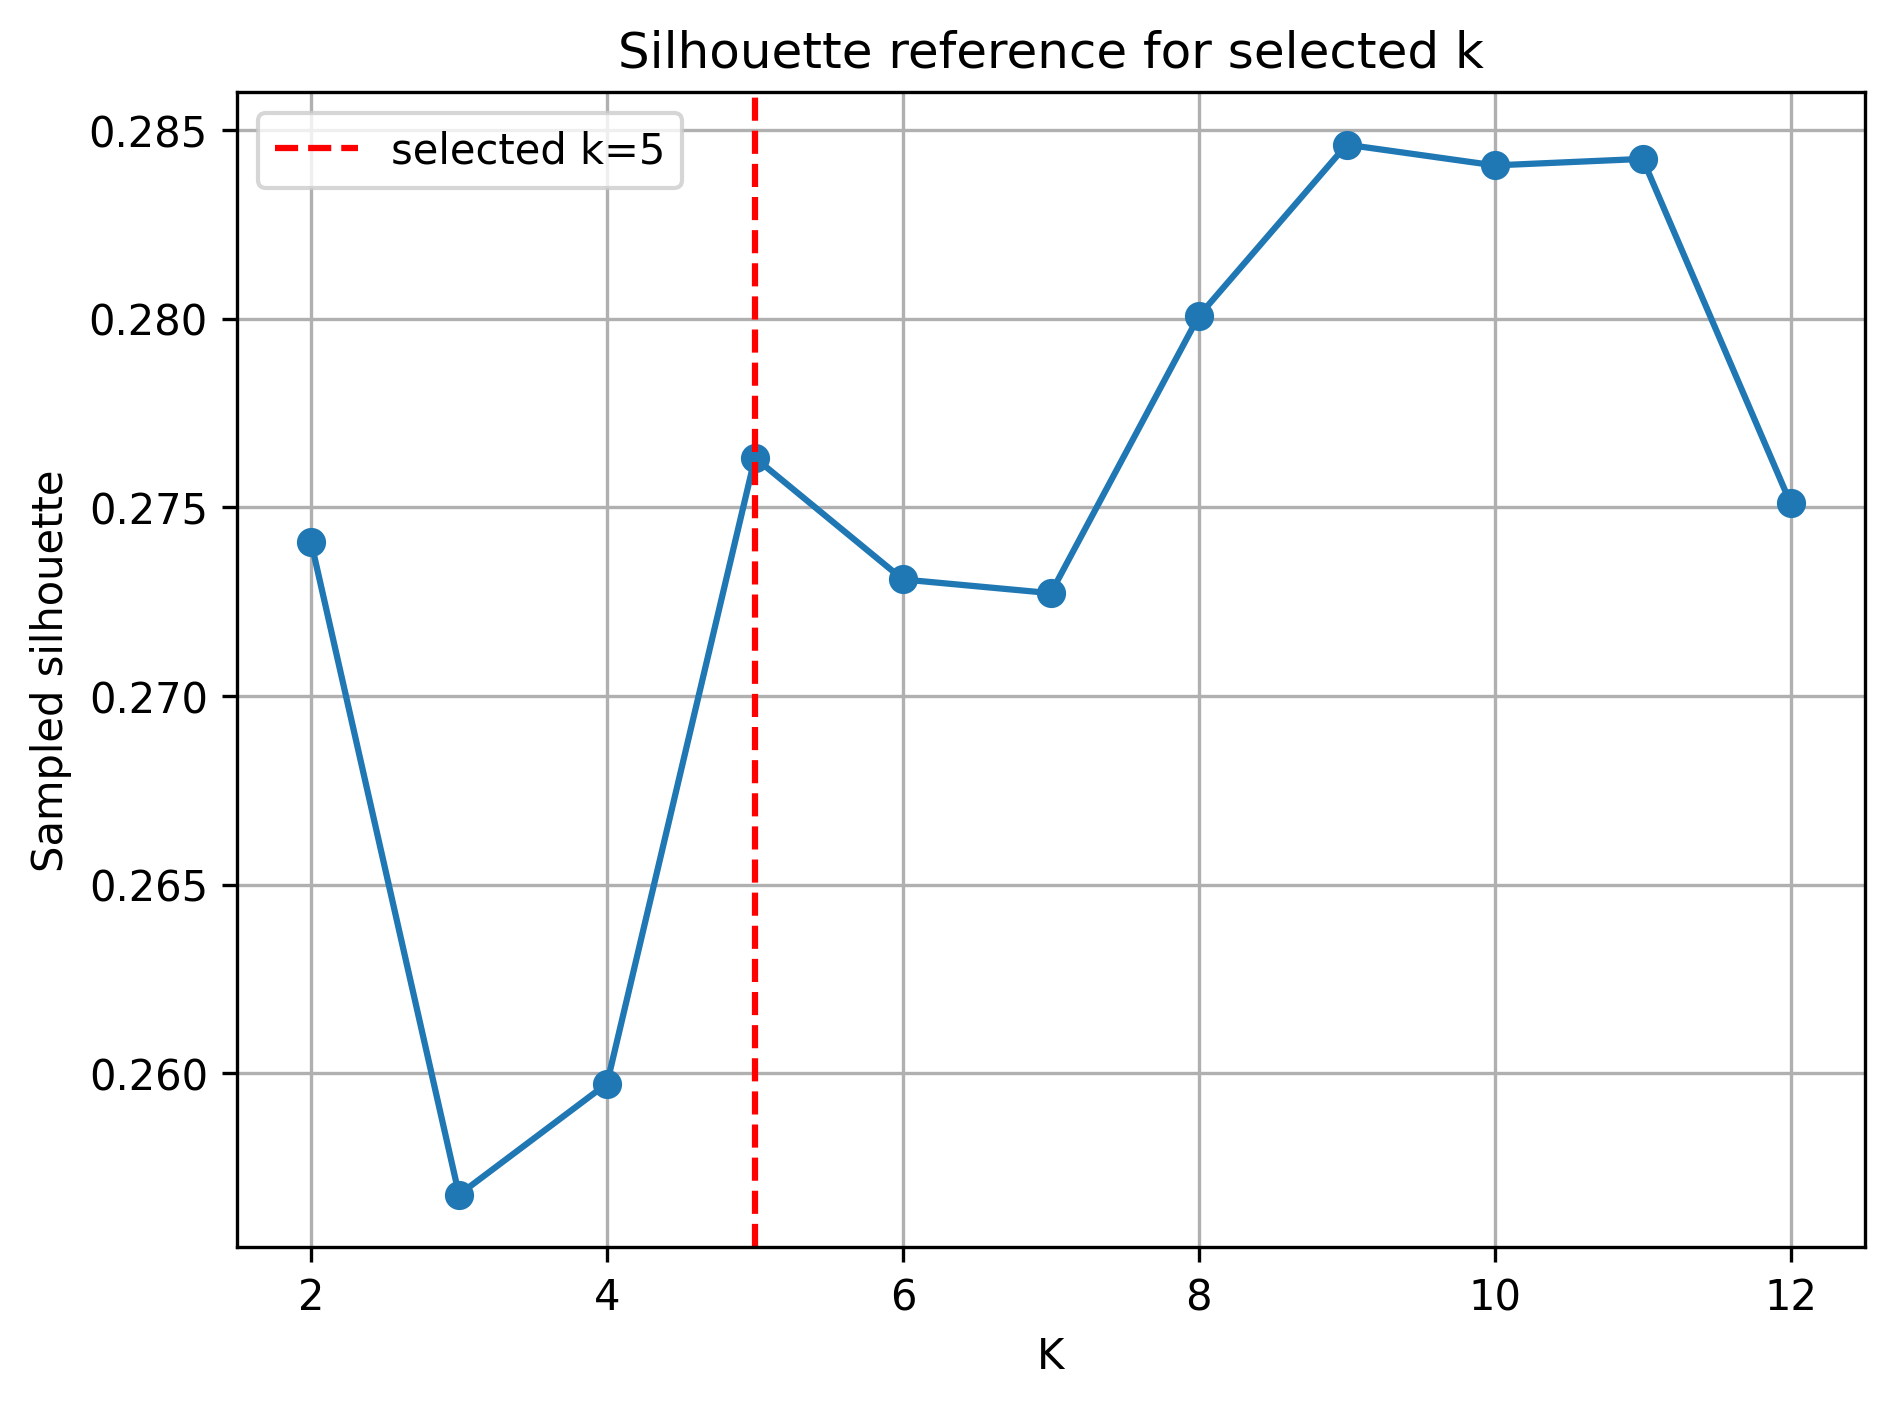
\includegraphics[width=\linewidth]{figures/cluster-count-silhouette.png}
\caption{Sampled silhouette scores for reference.}
\end{subfigure}
\caption[Cluster-count selection in the pretrained spectrogram latent space]{Cluster-count diagnostics for K-means in the 32-dimensional pretrained spectrogram latent space, before DEC refinement. (a) Log inertia for candidate counts \(K=2,\ldots,12\); the normalized elbow criterion selects \(K=5\). (b) Sampled silhouette scores for the same candidate counts, shown only as supplementary information rather than as the selection criterion. The red dashed line marks the elbow-selected count in both panels.}
\label{fig:cluster-count-selection}
\end{figure}

\subsection{Deep Clustering Refinement with a Reconstruction Constraint}

Clustering refinement follows the soft-assignment and target-distribution update procedure of DEC. Given particle features \(z_i\) and cluster centers \(\mu_j\), soft assignments are calculated using Student's t-distribution:

\begin{equation} q_{ij} = \frac{ \left(1+\|z_i-\mu_j\|_2^2/\alpha\right)^{-(\alpha+1)/2} }{ \displaystyle\sum_{k=1}^{K} \left(1+\|z_i-\mu_k\|_2^2/\alpha\right)^{-(\alpha+1)/2} }, \qquad \alpha=1. \end{equation}

Here, \(q_{ij}\) represents the soft assignment of particle \(i\) to cluster \(j\), with assignments summing to one for each particle~\cite{xie2016}.

An auxiliary target distribution is constructed from the current assignments:

\begin{equation} f_j=\sum_{i=1}^{N}q_{ij}, \qquad p_{ij} = \frac{q_{ij}^{\,2}/f_j} {\displaystyle\sum_{k=1}^{K}q_{ik}^{\,2}/f_k}. \end{equation}

The quantity \(f_j\) is the total soft-assignment mass of cluster \(j\). Squaring the assignments emphasizes higher-confidence memberships, while normalization by cluster frequency adjusts the relative contributions of different clusters. The target distribution is calculated using all particles and updated after each epoch; it stays constant during the next epoch's gradient updates and is not included in backpropagation.

The decoder and reconstruction loss are retained during clustering refinement to constrain changes to the input representation. Combining reconstruction and clustering objectives follows the structure preservation approach introduced in IDEC~\cite{guo2017}.

The clustering loss for the current batch is

\begin{equation} L_{\mathrm{cluster}} = \sum_{i\in\mathcal{B}} \sum_{j=1}^{K} p_{ij}\log\frac{p_{ij}}{q_{ij}}. \end{equation}

The joint training objective is

\begin{equation} L = L_{\mathrm{recon}} + \lambda L_{\mathrm{cluster}}, \qquad \lambda=5\times10^{-4}. \end{equation}

The reconstruction term is the channel-weighted loss used during pretraining. The KL term is summed up over the particles and clusters in the present batch and not averaged over the particles, so its coefficient has to be understood in conjunction with the loss reduction and the batch size, which is fixed at 64.

This report uses the reconstruction-plus-weighted-clustering form used in the previous one. The coefficient chosen in this case resulted from exploratory comparisons of the clustering weights. Because of differences in input standardization, the weighting of the reconstruction, and the KL reduction, there is no direct numerical agreement with the coefficient given in the earlier study.

During refinement, a randomly chosen half of the particles---that is, 6,400 samples---participate in the gradient updates. For all 12,800 particles, the soft assignments and the target distributions are calculated both at the beginning of training and after each epoch. As a result, particles left out of the refinement gradient updates still help construct the target distributions and are not treated as an independent test set.

Refinement uses Adam with a learning rate of \(10^{-3}\). The reconstruction loss updates the encoder and decoder, while the clustering loss updates the encoder and cluster centers. Final labels are obtained from the soft assignments:

\begin{equation} y_i=\underset{j}{\arg\max}\;q_{ij}. \end{equation}

These discrete labels are used for output and monitoring and do not participate in gradient computation. Figure~\ref{fig:architecture} illustrates the model structure and these dependencies.

\begin{figure}[htbp]
\centering
\figureasset[\linewidth]{figures/architecture.png}{Convolutional autoencoder and reconstruction-constrained deep clustering}
\caption[Convolutional autoencoder and reconstruction-constrained deep clustering]{Convolutional autoencoder and deep clustering refinement with a reconstruction constraint. The encoder maps each six-channel spectrogram to a 32-dimensional representation, from which the decoder reconstructs the input. Latent features and cluster centers jointly determine soft assignments \(Q\), which are used to construct the auxiliary target distribution \(P\). Training combines a channel-weighted reconstruction loss with a KL clustering loss using \(\lambda=5\times10^{-4}\). The KL term is summed over minibatch particles and clusters. Reconstruction updates the encoder and decoder, while clustering updates the encoder and cluster centers. Final labels are obtained by selecting the largest soft assignment for each particle. Spectrograms, latent features, and cluster distributions in the diagram are schematic.}\label{fig:architecture}
\end{figure}

\subsection{Training Monitoring and Model Selection}

The final configuration performs 350 epochs of deep clustering refinement. Total loss, reconstruction loss, the unweighted KL term, and its weighted contribution are recorded at each epoch. Changes in particle assignments are also monitored.

The label-change rate between consecutive epochs is defined as

\begin{equation} \delta^{(t)} = \frac{1}{N} \sum_{i=1}^{N} \mathbf{1} \left[ y_i^{(t)}\neq y_i^{(t-1)} \right], \end{equation}

where \(\mathbf{1}[\cdot]\) is the indicator function. This metric gives the fraction of particles reassigned between consecutive epochs. Refinement runs for the prescribed number of epochs; the label-change rate is used as a diagnostic and does not trigger early stopping.

Following each epoch, the silhouette score is calculated by means of Euclidean distances within the present latent space, based on a subset of 5,000 particles that are selected using a fixed random seed. This score serves both as a means of monitoring the training process and as a basis for model selection, with the candidate that has the highest score being kept. The score's interpretation with regard to within-cluster cohesion and between-cluster separation is in accordance with Rousseeuw's definition~\cite{rousseeuw1987}.

Once the model has been selected, final labels are assigned to all the particles, and the silhouette score is then recalculated on a subset consisting of 10,000 particles. It is for this reason that the final score reported might differ slightly from the score obtained during epoch-level monitoring. Since the model selection and the final evaluation both make use of the same analysis dataset, these scores are given as internal clustering assessments and not as independent test results.

The workflow keeps the representations and labels that were obtained before refinement, along with the losses at each epoch and the changes in assignment. The final outputs consist of the particle identifiers, the cluster labels, the latent features, the sampling settings, and the loss weights, which enable the assignments to be linked to the original trajectories. The key settings are given in Table~\ref{tab:settings} in Appendix~\ref{app:implementation}.

\clearpage
\section{Experimental Design}\label{sec:experiments}

\subsection{Objectives and General Settings}

Two comparative experiments are carried out to evaluate the spectrogram-based deep clustering workflow for multivariate particle trajectories. The first uses principal component analysis (PCA) followed by K-means as a linear dimensionality reduction baseline. The second applies a one-dimensional convolutional autoencoder followed by DEC directly to multichannel time series, and this provides a reference for comparison with the time--frequency representation used by the main method.

All methods use the same 12,800 particles and six input channels: position \(x\), momentum components \(p_x\) and \(p_y\), and local electromagnetic field components \(E_x\), \(E_y\), and \(B_z\). The same temporal sampling indices are used for all channels, which results in 2,004 evenly spaced samples per particle. For the time-series standardization, the mean values and standard deviations are calculated for each channel across all particles and at the chosen time points. These normalization parameters are used in all the experiments.

The representation dimension used for clustering is fixed at 32 for all methods. Since the spectrogram workflow employs the elbow criterion and selects five clusters, the comparative experiments also use \(K=5\). A fixed random seed of 42 is used, and the final silhouette evaluation is performed on the same subset of 10,000 particles, aligned by particle ID.

\subsection{Compared Methods}

The input representations, dimensionality reduction procedures, and clustering stages are summarized in Table~\ref{tab:methods}.

\begin{table}[htbp]
\centering\small
\caption{Input representations and clustering procedures of the compared methods. All clustering representations have 32 dimensions.}\label{tab:methods}
\begin{tabularx}{\linewidth}{@{}p{0.18\linewidth}Y Y Y@{}}
\toprule
\textbf{Method} & \textbf{Input} & \textbf{Representation construction} & \textbf{Clustering} \\
\midrule
PCA + K-means & Six-channel spectrograms & Flattening followed by PCA & K-means \\
1D CNN + DEC & Six-channel standardized time series & One-dimensional convolutional autoencoder & K-means initialization followed by DEC refinement \\
Spectrogram CNN + DEC & Six-channel spectrograms & Two-dimensional convolutional autoencoder & K-means initialization followed by DEC refinement \\
\bottomrule
\end{tabularx}
\end{table}

\noindent\textbf{PCA + K-means.} This baseline uses the same spectrogram preprocessing as the main method, including time-series standardization, spectrogram computation, logarithmic transformation, resizing, and spectrogram standardization. Each particle is represented by a spectrogram tensor of size \(6\times33\times60\), which is flattened into an 11,880-dimensional vector.

PCA reduces this vector to 32 dimensions without whitening. K-means then partitions the resulting representations into five clusters. Both PCA and K-means are fitted using all particles. K-means uses 100 initializations and a maximum of 1,000 iterations.

This experiment provides a baseline that does not require neural network training. Clustering is evaluated primarily through the silhouette score in the 32-dimensional PCA space.

\noindent\textbf{1D CNN + DEC.} This method directly takes standardized particle time series of size \(6\times2,004\) as input. To do this, the encoder uses four one-dimensional convolutional layers to extract temporal features and then transforms them into a 32-dimensional latent vector. The decoder then reconstructs the six-channel time series from this representation.

After autoencoder pretraining, K-means initializes five cluster centers in the latent space. Then, DEC improves the representation and cluster centers through optimization, which is carried out jointly on reconstruction and clustering. The final cluster labels are derived from the soft assignments of the chosen model.

This experiment provides a deep learning reference that operates directly on multichannel time series. Its convolutional depth and channel widths correspond to those of the spectrogram network, while the latent dimension and principal training settings are shared. Because the input shapes and convolutional operations differ, the two networks do not have identical parameter counts. The comparison therefore concerns the complete input representations and their corresponding network configurations.

\noindent\textbf{Spectrogram CNN + DEC.} This is the study's main method. The six-channel particle time series are transformed into multichannel spectrograms, and then a two-dimensional convolutional autoencoder learns 32-dimensional representations. K-means initializes the cluster centers, and DEC then updates the network parameters and cluster centers.

The preprocessing, network architecture, and joint optimization objective are described in the Methods section. The final training configuration is used for comparison with the two reference methods.

\subsection{Training Settings for the Deep Models}

Both convolutional models are trained in two stages: autoencoder pretraining and clustering refinement.

During pretraining, 80\% of the particles are used to optimize the autoencoder, and the remaining 20\% are used to monitor reconstruction loss. Training runs for a maximum of 200 epochs and stops if the validation reconstruction loss does not improve for 15 consecutive epochs. The model weights corresponding to the lowest validation loss are restored. Both models use the Adam optimizer with a learning rate of \(10^{-3}\) and a batch size of 64.

The reconstruction objective is a channel-weighted mean squared error. For the channel order \(x\), \(p_x\), \(p_y\), \(E_x\), \(E_y\), \(B_z\), the weights are

\begin{equation} \boldsymbol{w}=(1,\;1,\;1,\;0.2,\;0.2,\;1). \end{equation}

The squared reconstruction errors are multiplied by their channel weights, averaged over all elements in the minibatch, and divided by the mean channel weight. This maintains the reconstruction-loss definition used by the main method.

During DEC refinement, the joint objective is

\begin{equation} L=L_{\mathrm{recon}}+\lambda L_{\mathrm{cluster}}, \qquad \lambda=5\times10^{-4}. \end{equation}

Here, \(L_{\mathrm{cluster}}\) is the KL divergence summed over all particles and clusters within the current minibatch. Both deep models use the same clustering weight and batch size, preserving the interpretation of the clustering contribution to the objective.

Following the implementation of the main method, a fixed subset containing 50\% of the particles is used for gradient updates during DEC training. The target distribution is updated using the soft assignments of all particles. DEC also uses Adam with a learning rate of \(10^{-3}\), with a training budget of 350 epochs.

To monitor the latent-space silhouette score during DEC training and to select the model weights for final evaluation, a fixed number of 5,000 particles is used. As a result, the final results cited refer to the model that has been selected and need not be identical to those obtained at the final training epoch.

These data partitions control optimization and monitoring. Since normalization, cluster initialization, and target-distribution updates involve the full particle dataset, the reported scores constitute internal clustering evaluation on the available data.

\subsection{Primary Evaluation Metric}

The silhouette score is the primary clustering evaluation metric. For particle \(i\), it is defined as

\begin{equation} s(i)=\frac{b(i)-a(i)} {\max\{a(i),b(i)\}}, \end{equation}

where \(a(i)\) is the mean distance between particle \(i\) and the other particles in its cluster. The quantity \(b(i)\) is the smallest mean distance between particle \(i\) and the particles belonging to any other cluster. The overall score is the average over the evaluation sample:

\begin{equation} S=\frac{1}{N_{\mathrm{eval}}} \sum_{i=1}^{N_{\mathrm{eval}}}s(i). \end{equation}

Higher scores indicate greater within-cluster cohesion and between-cluster separation under the chosen representation and distance metric.

To keep computational cost down while maintaining a consistent evaluation sample, all methods use the same 10,000 particles, selected with a fixed random seed. The Euclidean distance is used throughout, and both the within-cluster and between-cluster mean distances are computed within this sample. The evaluation spaces are:

\begin{itemize}
\item PCA + K-means: the 32-dimensional PCA representation.

\item 1D CNN + DEC: the 32-dimensional latent representation of the selected time-series model.

\item Spectrogram CNN + DEC: the 32-dimensional latent representation of the selected spectrogram model.
\end{itemize}

The report therefore includes the internal clustering scores within each method's own representation space, and the relevant evaluation space is specified in the results table. Classification accuracy is not given since the predefined particle-class labels are not available.

\subsection{Presentation of Results}

The main results are given in a table that compares the silhouette scores of the three methods, along with the representation dimension, cluster count, evaluation sample size, and measured end-to-end runtimes of the two deep workflows.

\clearpage
\section{Results and Analysis}\label{sec:results}

\subsection{Comparison of Clustering Scores and Runtime}\label{sec:silhouette-results}

The silhouette scores of the three methods and the measured end-to-end runtimes of the two deep workflows are summarized in Table~\ref{tab:silhouette}. All methods use the same six-channel particle data, a 32-dimensional representation, and five clusters. Evaluation is performed on the same subset of 10,000 particles.

\begin{table}[htbp]
\centering\small
\caption{Silhouette scores and end-to-end runtimes. Scores use Euclidean distance on the same sample of 10,000 particles, within each method's own 32-dimensional representation space. Runtimes were measured for 12,800 particles on an NVIDIA RTX PRO 6000 Blackwell Server Edition GPU and include preprocessing, autoencoder pretraining, 350 refinement epochs, evaluation, and figure generation. The PCA baseline runtime was not measured.}\label{tab:silhouette}
\begin{tabularx}{\linewidth}{@{}p{0.21\linewidth}Y c c r r@{}}
\toprule
\textbf{Method} & \textbf{Evaluation space} & \textbf{\shortstack{Latent\\dim.}} & \textbf{$K$} & \textbf{Silhouette} & \textbf{\shortstack{Runtime\\(s)}} \\
\midrule
PCA + K-means & PCA representation & 32 & 5 & 0.29957 & --- \\
1D CNN + DEC & Time-series latent space & 32 & 5 & 0.79637 & 405.19 \\
\shortstack[l]{Spectrogram CNN\\+ DEC} & Spectrogram latent space & 32 & 5 & 0.87985 & 524.62 \\
\bottomrule
\end{tabularx}
\end{table}

PCA + K-means achieves a silhouette score of 0.29957. It obtains this result by applying a linear projection to compress the spectrogram input before carrying out the clustering, and thus provides a baseline for comparison with the deep learning methods.

The 1D CNN + DEC method, by dealing directly with multichannel time series, attains a silhouette score of 0.79637. The fact that this score is higher shows that, with the current setup, the combination of one-dimensional convolutional representation learning and clustering refinement results in a representation that has a higher internal clustering score than the PCA baseline.

The version that uses Spectrogram CNN together with DEC attains the highest silhouette score, which is 0.87985 and is about 0.08348 higher than the 1D result. Hence, with respect to the dataset and training settings examined in this case, the spectrogram-based approach achieves the best score for both within-cluster cohesion and between-cluster separation in its final representation space.

\subsection{Computational Cost and Scalability}

On the NVIDIA RTX PRO 6000 Blackwell Server Edition GPU, end-to-end runtimes for 12,800 particles were 524.62~s for the spectrogram-based workflow and 405.19~s for the 1D time-series workflow. These measurements include preprocessing, autoencoder pretraining, 350 epochs of clustering refinement, evaluation, and figure generation. In the future, using the spectrogram-based workflow on larger PIC datasets with one to ten million tracked particles would need considerably more computational resources. Assuming approximately linear scaling with the number of particles and unchanged per-particle input dimensions and training settings, the estimated run time would be around 11.4 hours for one million particles and 4.7 days for ten million particles on the same hardware. These estimates give a first indication of the computational cost; actual deployment at this scale would also demand efficient data loading and memory management.

\subsection{Training Process of the Spectrogram Method}

The training curves provide supplementary information about the optimization of the main method. Figure~\ref{fig:training} shows the training and validation reconstruction losses during autoencoder pretraining, the loss components during DEC refinement, and the latent-space silhouette monitored during refinement.

\begin{figure}[htbp]
\centering
\begin{subfigure}[t]{0.48\linewidth}
\centering
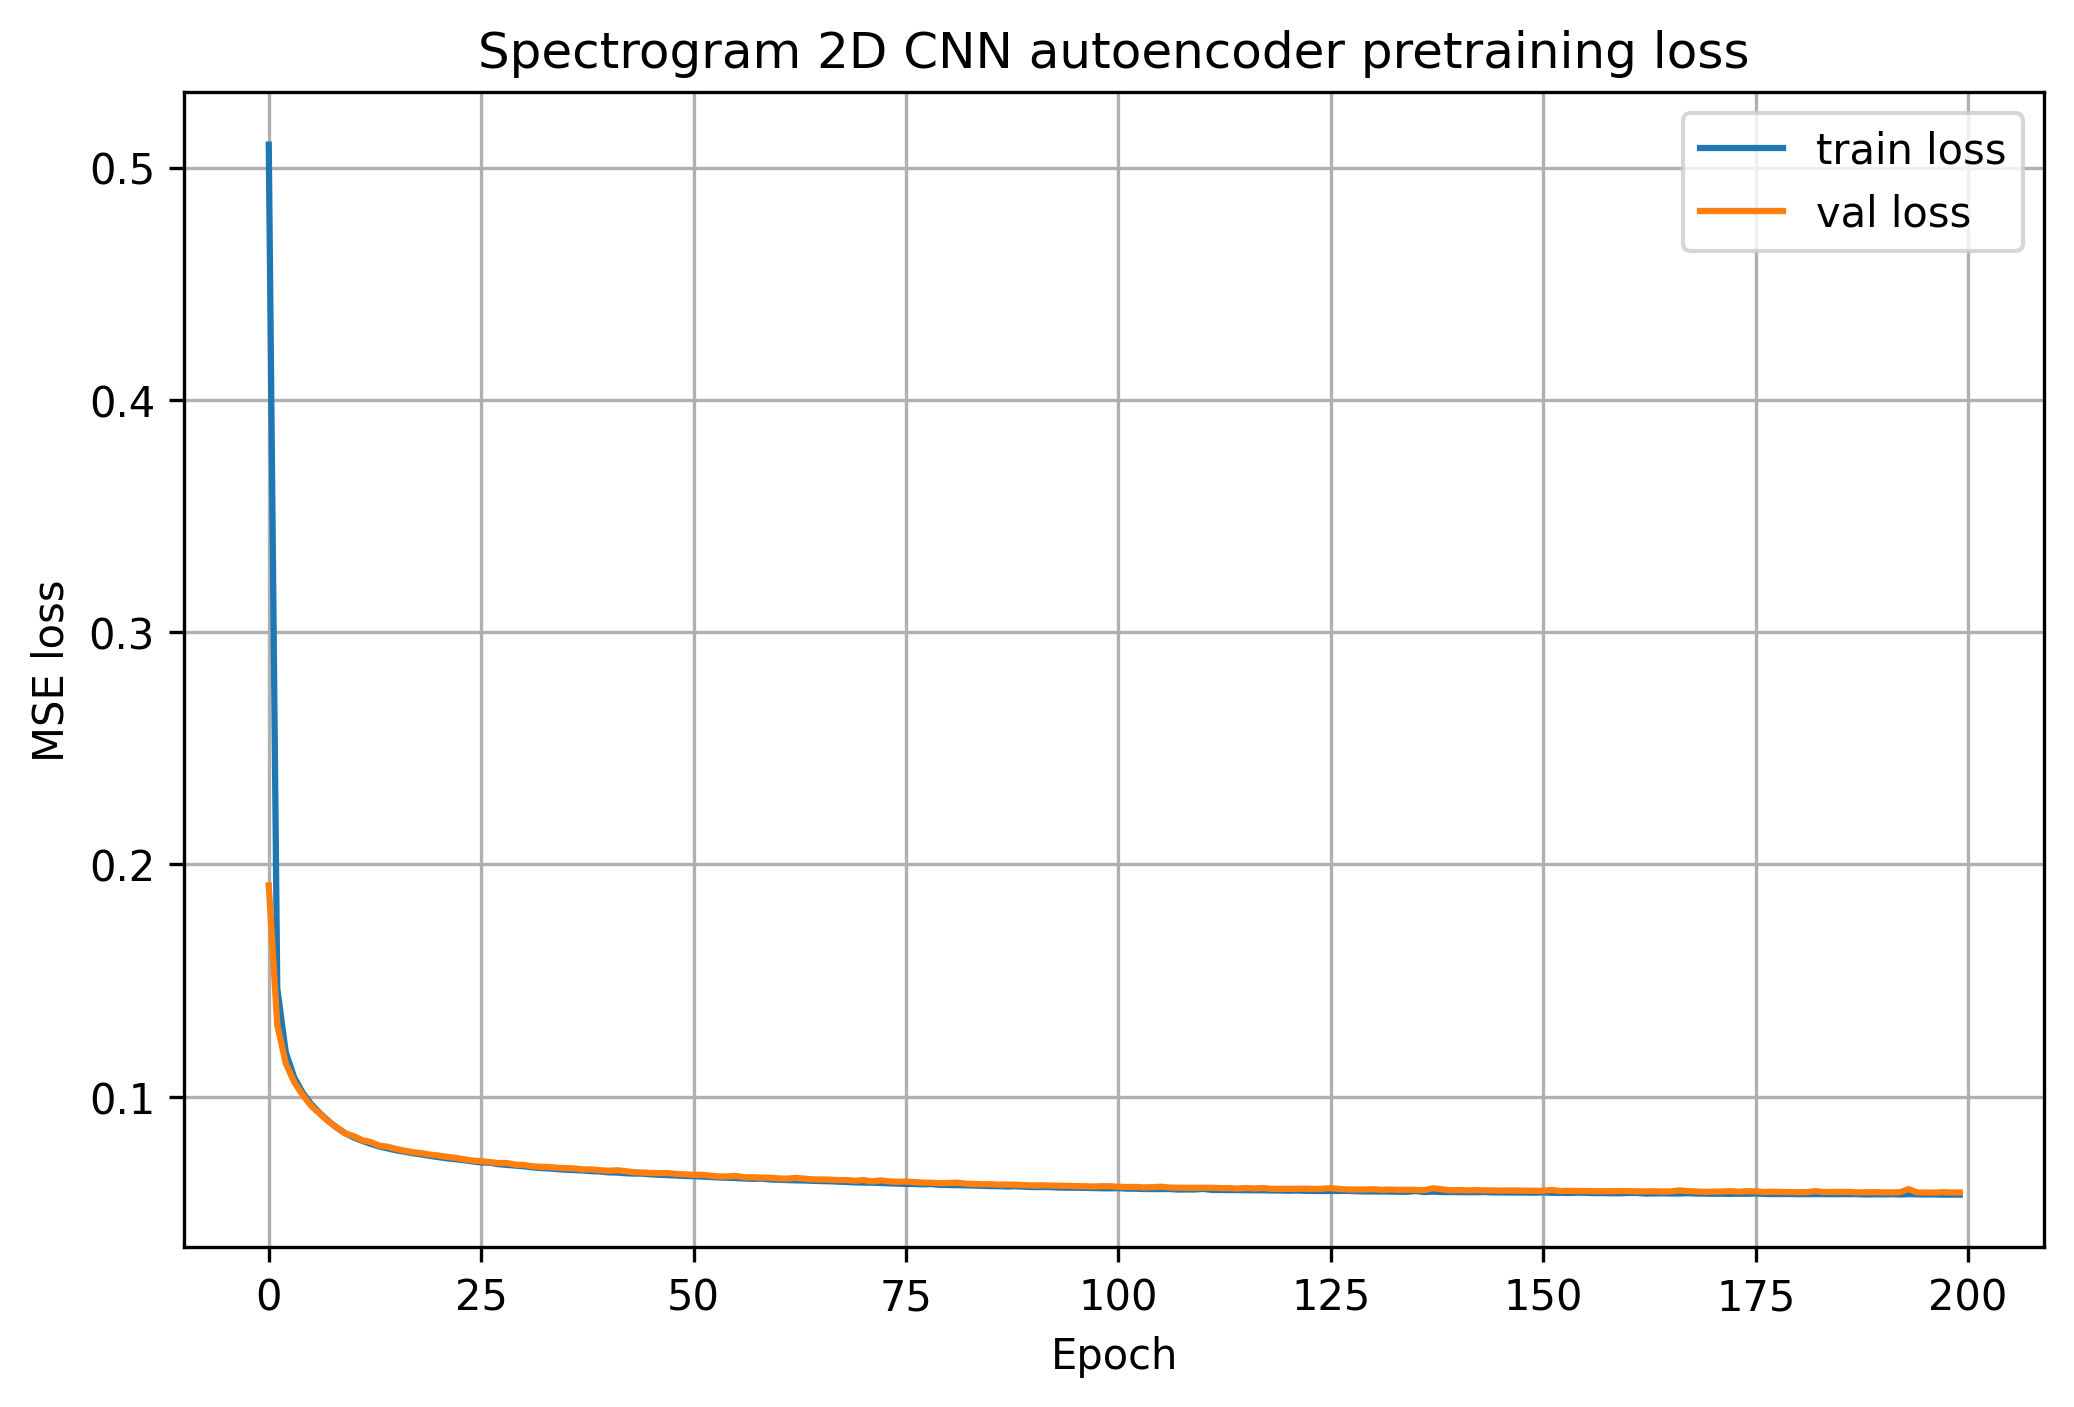
\includegraphics[width=\linewidth]{figures/ae-pretraining-loss.png}
\caption{Pretraining reconstruction losses.}
\end{subfigure}\hfill
\begin{subfigure}[t]{0.48\linewidth}
\centering
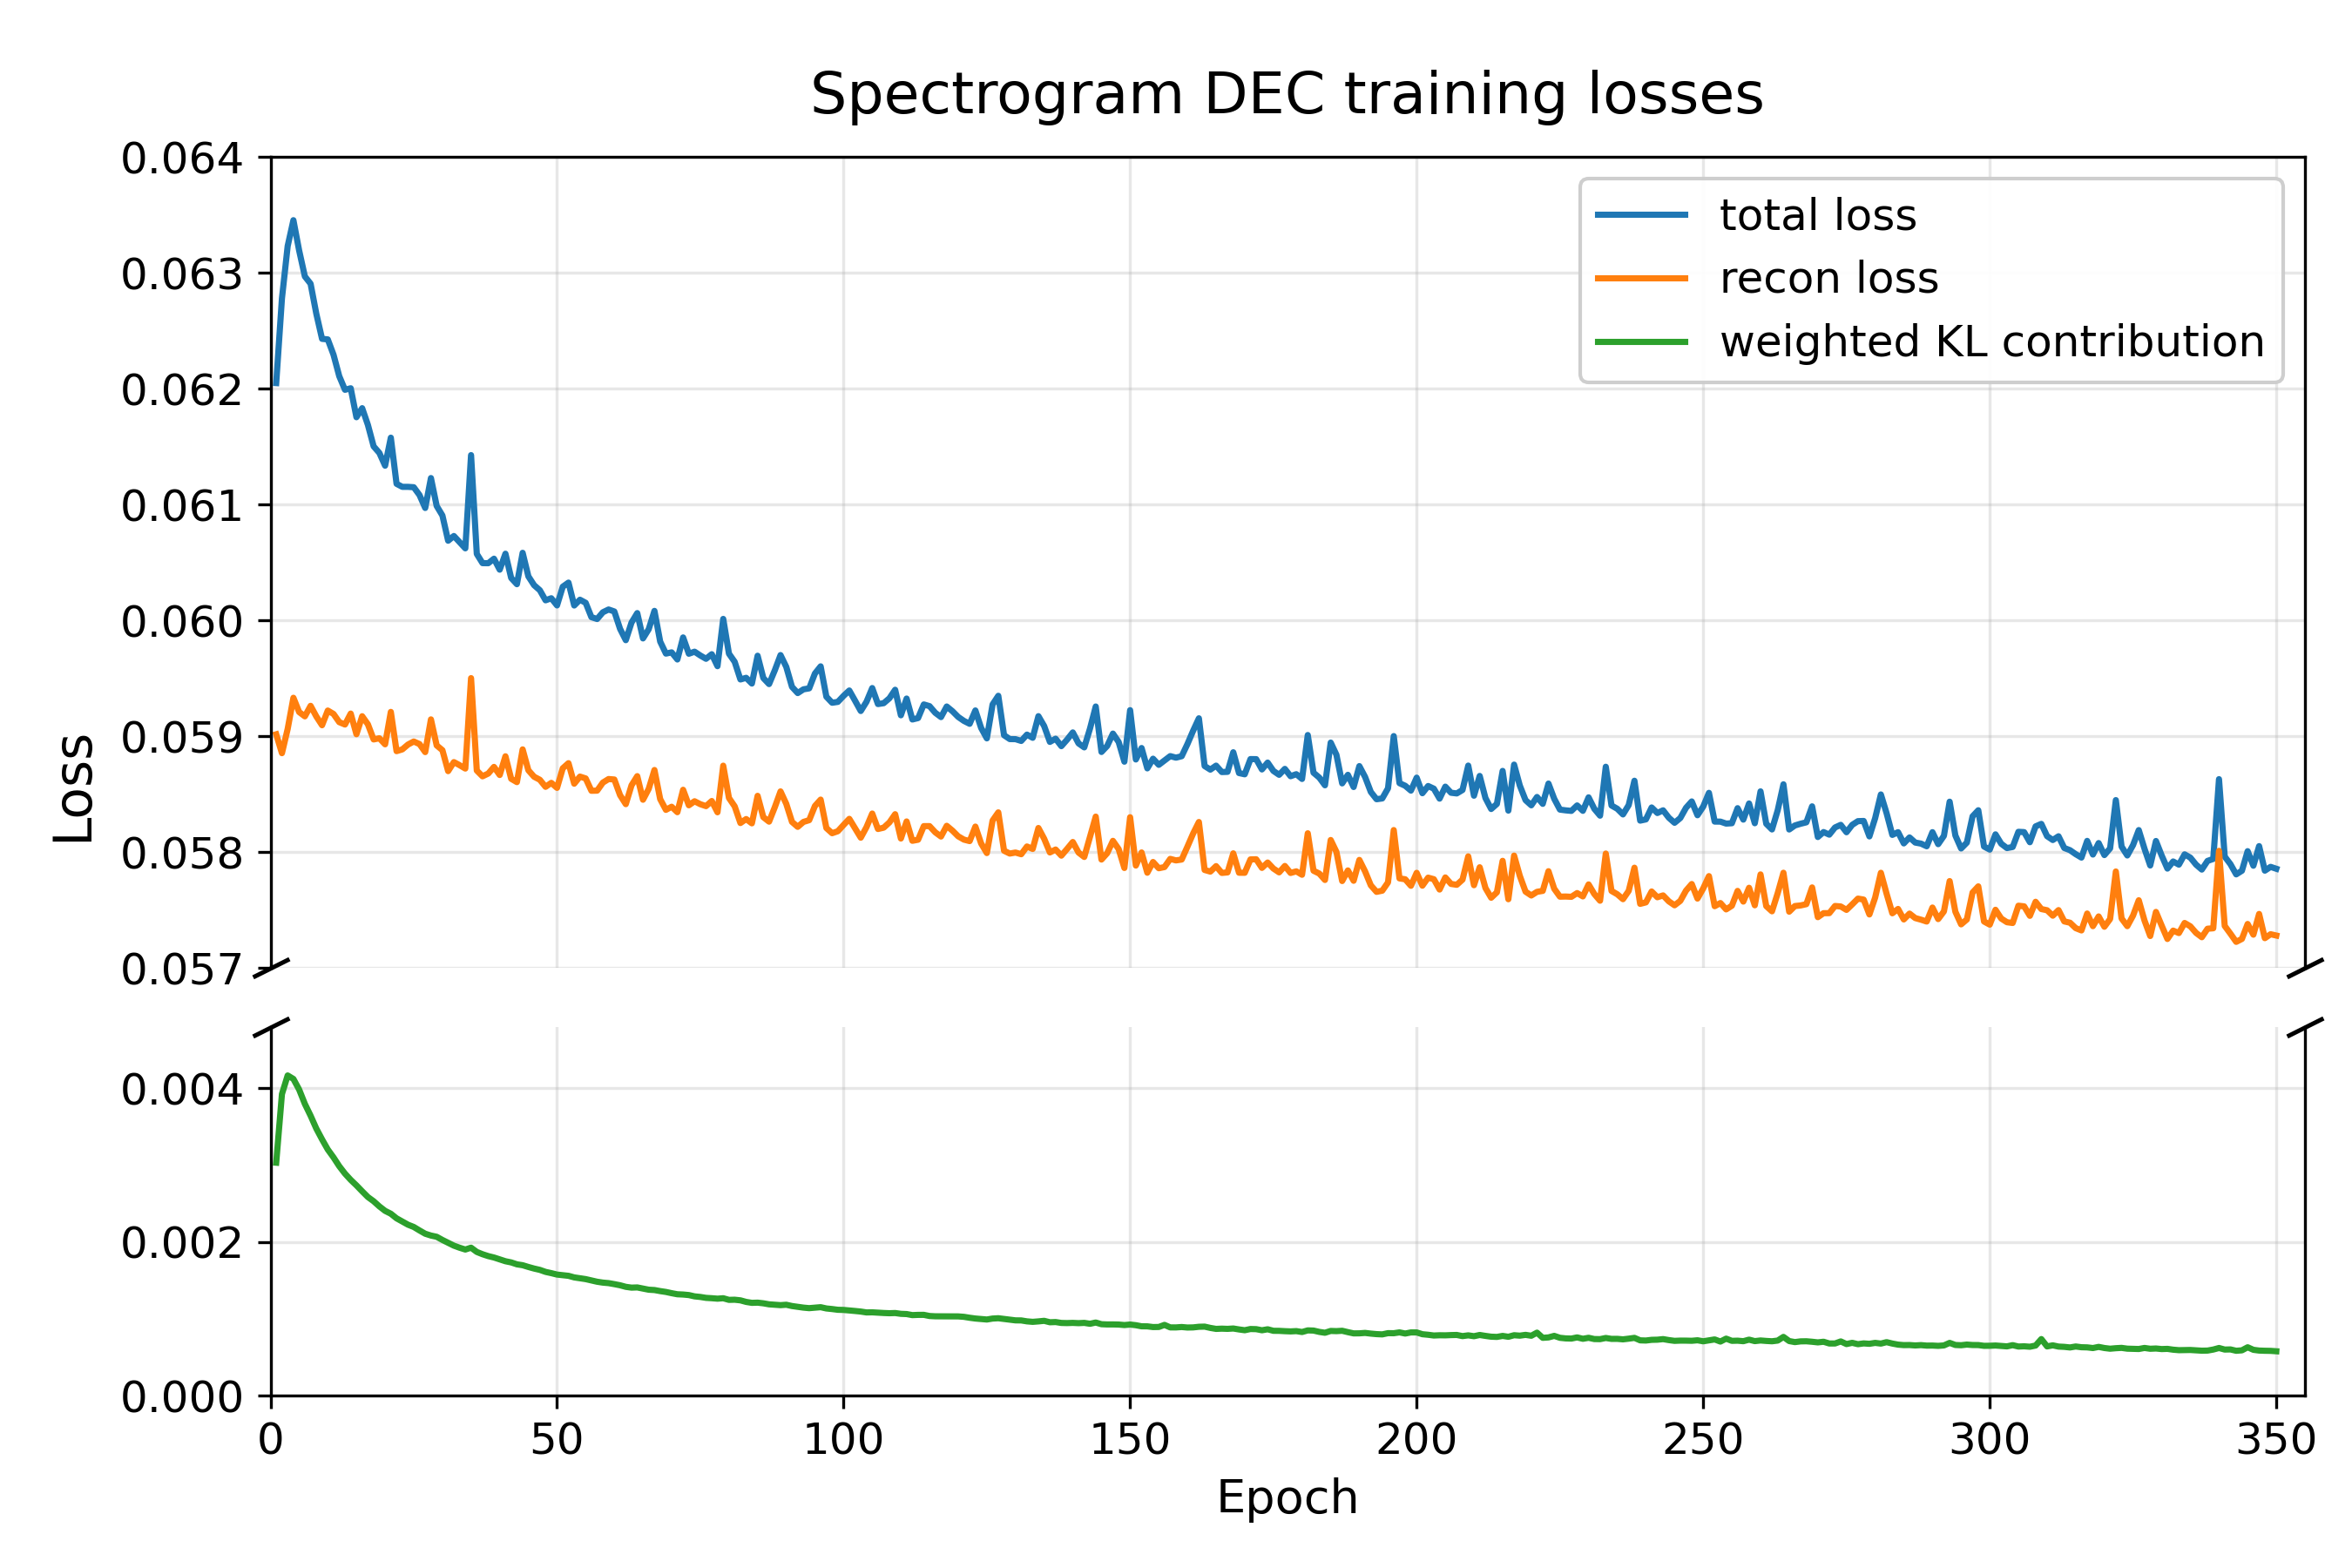
\includegraphics[width=\linewidth]{figures/dec-training-loss-zoomed.png}
\caption{DEC refinement losses with a broken vertical axis.}
\end{subfigure}
\par\medskip
\begin{subfigure}[t]{0.48\linewidth}
\centering
\figureasset[\linewidth]{figures/dec-silhouette.png}{Latent-space silhouette}
\caption{Latent-space silhouette.}
\end{subfigure}
\caption[Training and monitoring diagnostics for the spectrogram method]{Training and monitoring diagnostics for the spectrogram method. (a) Training and validation reconstruction losses during autoencoder pretraining. (b) Total loss, reconstruction loss, and the weighted KL contribution during DEC refinement. (c) Latent-space silhouette during refinement. Training-time silhouette monitoring uses a fixed sample of 5,000 particles, while final evaluation uses 10,000 particles.}
\label{fig:training}
\end{figure}

In the early epochs of pretraining, the training and validation reconstruction losses drop quickly and then fall off more slowly, staying nearly the same for the majority of the training process. These losses are used to monitor learning and to select the autoencoder weights for the clustering phase. DEC then jointly optimizes both the reconstruction and clustering objectives, updating both the representation and the cluster centers. After this initial transient period, the total loss and the weighted KL term both decrease, while the reconstruction loss changes more slowly. The monitored latent-space silhouette rises as the process is refined.

The clustering term is defined as the KL divergence summed over the current minibatch and weighted by \(5\times10^{-4}\). Since the loss plot displays the weighted KL contribution, the numerical size of this component can be compared with that of the reconstruction term. However, the coefficient must be interpreted in light of the loss-reduction convention, since its magnitude alone does not indicate the extent to which clustering optimization affects the result.

The main method carries out 350 DEC training epochs. During training, the silhouette score uses a fixed sample of 5,000 particles, while the final evaluation uses 10,000 particles. As a result, the scores obtained during monitoring and at the end need not be the same. The final evaluation also uses the selected model weights, and these weights do not necessarily correspond to the last training epoch.

These curves describe the optimization and model-selection process. The comparison between methods remains based on the final scores obtained using the common evaluation sample in Section~\ref{sec:silhouette-results}.

\FloatBarrier
\subsection{Reconstruction of the Six-Channel Spectrograms}

To show how the autoencoder reconstructs data, the input and reconstructed spectrograms for a particular particle are displayed side by side for all six channels. The reconstruction uses the pretrained model with the lowest validation reconstruction loss. Figure~\ref{fig:reconstruction} shows this comparison.

\begin{figure}[htbp]
\centering
\figureasset[0.83\linewidth]{figures/reconstruction.png}{Six-channel spectrogram reconstruction}
\caption[Six-channel spectrogram reconstruction]{Six-channel spectrogram reconstruction by the pretrained autoencoder. The left column shows the input spectrograms of a selected particle, and the right column shows the corresponding reconstructions. Rows represent the \(x\), \(p_x\), \(p_y\), \(E_x\), \(E_y\), and \(B_z\) channels, respectively. Reconstructions are obtained from the pretrained model with the lowest validation reconstruction loss.}\label{fig:reconstruction}
\end{figure}

The six channels describe particle position, momentum components, and local electromagnetic field components. The paired display provides a visual comparison between the input and reconstruction for each channel, so that differences in spectral distributions and local details can be examined.

Reconstruction and silhouette evaluate different aspects of the model. Reconstruction measures the autoencoder's ability to reproduce its input, while silhouette reflects the grouping structure in the chosen representation space. Reconstruction is therefore employed as a supplementary diagnostic rather than as a direct criterion for assessing clustering quality.

\subsection{Visualization of the Final Clustering}

The final 32-dimensional representations of the spectrogram method are projected into two dimensions using PCA and t-SNE. Particles are colored according to their final cluster assignments. Figure~\ref{fig:latent-projections} shows both projections.

\begin{figure}[htbp]
\centering
\begin{subfigure}[t]{0.49\linewidth}
\centering
\figureasset[\linewidth]{figures/latent-pca.png}{PCA projection}
\caption{PCA projection.}
\end{subfigure}\hfill
\begin{subfigure}[t]{0.49\linewidth}
\centering
\figureasset[\linewidth]{figures/latent-tsne.png}{t-SNE projection}
\caption{t-SNE projection.}
\end{subfigure}
\caption[Two-dimensional projections of the final latent representations]{Two-dimensional visualization of the final spectrogram CNN + DEC representations. Colors indicate the five final cluster assignments. Clustering and silhouette evaluation are performed in the 32-dimensional latent space; the two-dimensional projections are used only for visualization.}
\label{fig:latent-projections}
\end{figure}

The PCA projection provides a linear view of the latent distribution, and the t-SNE projection offers a supplementary visualization of local neighborhood relationships. Both plots use the previously obtained final labels; clustering is not repeated in the two-dimensional coordinates.

These visualizations allow a qualitative examination of how the clusters are distributed. Because a two-dimensional projection retains only part of the high-dimensional structure, visual distances do not directly correspond to distances in the full latent space. The silhouette score was calculated using all 32 latent dimensions.

\subsection{Final Cluster Sizes}

The main method partitions the 12,800 particles into five nonempty clusters. Their sizes and proportions are listed in Table~\ref{tab:cluster-sizes} in Appendix~\ref{app:clusters}.

The largest group consists of 3,884 particles (30.34\% of the dataset), and the smallest group has 1,818 particles (14.20\%). Each of the five clusters includes a large number of particles, with no empty clusters and no clusters with only a small number of particles.

The cluster-size distribution supplements the silhouette evaluation by describing how particles are distributed among the groups. Cluster size alone does not establish the correctness of a partition, nor does the clustering objective require equally sized groups.
\clearpage
\section{Conclusions, Limitations, and Implications}\label{sec:conclusions}

\subsection{Conclusions}

The study presents an unsupervised procedure that uses time--frequency representations and convolutional deep clustering to analyze multivariate particle trajectories from particle-in-cell (PIC) simulations. Extending earlier research on clustering particle trajectories, the input now includes six channels: particle position, momentum components, and local electromagnetic field components. After carrying out uniform temporal sampling and standardization, the channels are converted into spectrograms. A two-dimensional convolutional autoencoder produces low-dimensional representations, and the particle groups are determined by first using K-means initialization and then refining them with DEC.

When the silhouette is used as the evaluation criterion, the spectrogram CNN + DEC method is compared with PCA + K-means and the 1D time-series CNN + DEC. All three methods use 32-dimensional representations and five clusters, and the evaluation is performed on the same sample of 10,000 particles. The silhouette scores obtained for PCA + K-means, 1D CNN + DEC, and spectrogram CNN + DEC are 0.29957, 0.79637, and 0.87985, respectively. The spectrogram-based method achieves the highest internal clustering score in its representation space among all methods investigated.

The results show that spectrogram-based convolutional deep clustering is a viable method for organizing multivariate PIC particle trajectories. The procedure converts high-dimensional, multichannel particle recordings into low-dimensional representations suitable for grouping and retrieval, without requiring predefined class labels. Furthermore, the training curves, spectrogram reconstructions, latent-space projections, and cluster sizes provide additional descriptions of the model's behavior and outputs.

\subsection{Limitations}

The assessment is mainly based on the silhouette score. This criterion captures both cohesion within clusters and separation between clusters for a given representation and distance measure, although it does not directly show that particle groups correspond to the true categories. As each technique is evaluated within its own representation space, the comparison shows the internal clustering structure of those representations.

The experiments are based on the one available PIC particle dataset. They have not been carried out under other simulation conditions, time intervals, or with different particle samples. All steps involved in data standardization, cluster initialization, and updating the DEC target distribution use the existing dataset. Therefore, the results here represent an internal evaluation using the available data and do not prove the ability to generalize to new data.

Spectrogram preprocessing also involves certain compromises in representation. To create inputs of a uniform shape, we use logarithmic magnitude spectrograms along with resizing. This representation does not explicitly preserve all phase information and may lose some local details. As a result, the resulting groups depend on the chosen channels, the sampling method, and the spectrogram parameters, and therefore should not be considered the only possible way to divide particle trajectories.

\subsection{Implications and Potential Applications}

The study sets out a computational procedure for turning the outputs of multivariate simulations into particle groups which can then be used in further analysis. When it is impractical to examine each particle record individually, cluster labels can serve as an indexing tool for organization, enabling researchers to browse trajectories by group, draw representative samples, and compare variable distributions across groups. This organization provides a structured basis for further analysis and reduces the need to manually examine individual trajectories.

Combining information on position, momentum, and the local electromagnetic field also provides a reusable method for analyzing particle data from multiple channels. A continuous processing workflow is established through uniform sampling, standardization, representation learning, and clustering evaluation. Saving the preprocessing parameters, model weights, and particle labels enables result verification and subsequent reuse.

In this study, clustering organizes particle records using computational methods. The resulting groups can then serve as inputs for domain-specific downstream analyses, enabling researchers to select the particle populations they want to examine in more detail. Ultimately, the value of these groups depends on whether they support those later tasks efficiently, in addition to the value of a single clustering metric.

\section{Declaration of AI Assistance}\label{sec:ai-assistance}

OpenAI's ChatGPT was used to assist with identifying relevant literature, planning experimental workflows, correcting grammatical errors, improving the clarity and readability of the manuscript, and preparing LaTeX formatting. It also assisted with developing and debugging code for supplementary experiments.

\clearpage
\phantomsection
\addcontentsline{toc}{section}{References}
\bibliographystyle{unsrtnat}
\bibliography{references}

\clearpage
\appendix
\renewcommand{\thetable}{\thesection.\arabic{table}}
\section{Architecture and Training Configuration}\label{app:implementation}
\setcounter{table}{0}

\subsection{Convolutional Autoencoder Architecture}

Table~\ref{tab:architecture} provides the layer-by-layer dimensions of the spectrogram autoencoder. Dimensions exclude the batch axis.

\begin{table}[htbp]
\centering\small
\caption{Main components of the convolutional autoencoder. Dimensions exclude the batch axis.}\label{tab:architecture}
\begin{tabularx}{\linewidth}{@{}p{0.24\linewidth}Y p{0.21\linewidth}@{}}
\toprule
\textbf{Stage} & \textbf{Operation} & \textbf{Output dimensions} \\
\midrule
Input & Six-channel spectrogram & \(6\times33\times60\) \\
Encoder layer 1 & Two-dimensional convolution + ReLU & \(8\times17\times30\) \\
Encoder layer 2 & Two-dimensional convolution + ReLU & \(16\times9\times15\) \\
Encoder layer 3 & Two-dimensional convolution + ReLU & \(32\times5\times8\) \\
Encoder layer 4 & Two-dimensional convolution + ReLU & \(64\times3\times4\) \\
Feature compression & Flattening + linear fully connected layer & 32 \\
Decoder input & Linear fully connected layer + reshaping & \(64\times3\times4\) \\
Decoder & Four transposed convolutional layers & \(6\times34\times50\) \\
Output resizing & Bilinear interpolation & \(6\times33\times60\) \\
\bottomrule
\end{tabularx}
\end{table}

\clearpage
\subsection{Workflow and Optimization Settings}

Table~\ref{tab:settings} consolidates the preprocessing, pretraining, initialization, refinement, and model-selection settings of the final workflow.

\begingroup\small
\begin{longtable}{@{}p{0.54\linewidth}p{0.4\linewidth}@{}}
\caption{Main settings of the final analysis workflow.}\label{tab:settings}\\
\toprule
\textbf{Parameter} & \textbf{Setting} \\
\midrule
\endfirsthead
\multicolumn{2}{l}{\small\itshape Table~\thetable{} (continued)}\\
\toprule
\textbf{Parameter} & \textbf{Setting} \\
\midrule
\endhead
\midrule
\multicolumn{2}{r}{\small Continued on next page}\\
\endfoot
\bottomrule
\endlastfoot
Time-series dimensions per particle & \(6\times2004\) \\
Spectrogram window length / hop size & 256 / 128 \\
Network input dimensions & \(6\times33\times60\) \\
Latent dimensionality & 32 \\
Autoencoder training / validation split & 80\% / 20\% \\
Maximum pretraining epochs / early-stopping patience & 200 / 15 \\
Pretraining and refinement optimizer & Adam \\
Pretraining and refinement learning rate & \(10^{-3}\) \\
Batch size & 64 \\
Candidate cluster counts & 2--12 \\
K-means initializations / maximum iterations & 100 / 1,000 \\
Cluster-count selection & Elbow of the normalized log-inertia curve \\
Particles used for refinement gradient updates & 6,400 \\
Particles used to construct target distributions & 12,800 \\
Clustering loss coefficient & \(5\times10^{-4}\) \\
KL reduction & Sum over minibatch particles and clusters \\
Refinement epochs & 350 \\
Monitoring / final silhouette sample size & 5,000 / 10,000 \\
Model-selection criterion & Highest monitoring silhouette score \\
\end{longtable}
\endgroup
\clearpage
\section{Final Cluster Statistics}\label{app:clusters}
\setcounter{table}{0}

The counts and percentages in Table~\ref{tab:cluster-sizes} refer to the final spectrogram CNN + DEC assignments for all 12,800 particles. Cluster indices are identifiers, not predefined physical categories.

\begin{table}[htbp]
\centering\small
\caption{Particle counts and proportions of the five final clusters obtained using spectrogram CNN + DEC.}\label{tab:cluster-sizes}
\begin{tabularx}{\linewidth}{@{}Y r r@{}}
\toprule
\textbf{Cluster} & \textbf{Number of particles} & \textbf{Percentage of all particles} \\
\midrule
C0 & 3,884 & 30.34\% \\
C1 & 2,314 & 18.08\% \\
C2 & 2,068 & 16.16\% \\
C3 & 1,818 & 14.20\% \\
C4 & 2,716 & 21.22\% \\
\midrule
Total & 12,800 & 100.00\% \\
\bottomrule
\end{tabularx}
\end{table}
\end{document}
